\chapter{Valutazione retrospettiva}
\textit{Il seguente capitolo è dedicato ad illustrare i risultati ottenuti durante lo stage universitario. In aggiunta, è descritta la tecnologia adottata nello sviluppo del configuratore catalogo/prodotti.}

\section{\inde}
\inde\, come indicato dalla guida all'uso, ``é un [...] sistema di sviluppo che gestisce tutti gli aspetti del ciclo di vita del software, dall'analisi all'installazione ed oltre''\footcite{[11]}.
Questo strumento è una combinazione di più elementi: CASE, Framework ORM, RAD. Lo scopo ultimo di InDe è la creazione di Rich Internet Application compilate e tradotte sia in linguaggio Java che C\#, al fine di funzionare in qualsiasi server.
Le applicazioni web ideate seguono la programmazione relazionare, un modo di descrivere il comportamento del software tramite la composizione di un grafo di relazioni. I collegamenti si pongono l'obiettivo di mantenere conforme sia la struttura del database sia il codice generato. Questo fa si che ad ogni cambiamento a basso livello (ad esempio un attributo di una tabella cambia da intero a stringa), la modifica si propaghi in tutto il progetto fino ad esaurirsi.
Uno degli obiettivi della programmazione relazionale è quello di permettere ai programmatori di concentrare la propria attenzione sul prodotto finale senza doversi preoccupare degli aspetti tecnologici. La novità di questo tipo di programmazione è la gestione maggiore dei comportamenti della applicazione. Questa affermazione non esclude la programmazione tradizionale, la quale è perfettamente supportata.\\

In questa sezione andremo ad analizzare la metodologia alla base dello sviluppo e le tecnologie di sui compone \inde. Infine, viene presentata una breve guida alla creazione di una applicazione web.

\paragraph{RAD}\label{RAD}
RAD è una metodologia di sviluppo software, introdotta da James Martin negli anni '80. Come indicato su Wikipedia è una ``... metodologia [che] coinvolge modelli di sviluppo iterativi, la costruzione di prototipi e l'utilizzo di strumenti CASE''\footcite{[13]}. Essa prevede la creazione di rapida di prototipi e applicazioni. Tuttavia, la scalabilità del prodotto e il tempo a disposizione sono molto ridotti. InDe si basa su questa metodologia perché permette di creare velocemente prototipi e le applicazioni finali, ma per le tecnologie adottate ha risolto gli svantaggi.


\paragraph{CASE}\label{CASE}
I CASE (Computer Aided Software Engineering) sono strumenti software dedicati allo sviluppo assistito dal computer. Il primo risale agli anni '80. In generale, nelle software house, si predilige un'attività manuale, nella quale il ricorso a strumenti specializzati avviene solo nelle ultime fasi del processo attraverso l'uso di ambienti integrati (compilazione, linkaggio e debugging).
Tuttavia, dagli anni Ottanta ad oggi il loro sviluppo è proseguito, creando strumenti sofisticati come quelli che da diagrammi UML generano codice.
Lo scopo di questi strumenti è la gestione di complessità, modificabilità, qualità e automazione dei processi. I CASE permettono di generare codice e strutture dati di qualità. 

Gli strumenti CASE però non servono unicamente alla creazione di applicazione. Esistono categorie differenti di CASE mirati a semplificare una delle seguenti attività:
\begin{itemize}
	\item Progettazione (Access, Visio, Argo UML);
	\item Realizzazione del codice (Eclipse, Qt Creator);
	\item Supporto al controllo qualità (MaxQ, Suite Mercury);
	\item Supporto alla manutenzione (Erwin, Bugzilla);
	\item Gestione versioni e configurazioni (Subversion, Git);
	\item Pianificazione e gestione (Excel, Microsoft project, Asana);
\end{itemize}
I software citati nell'elenco precedente sono solo una piccola parte del vasto numero di software che oggi sono in circolazione. Tra questi programmi rientra anche \inde, il programma utilizzato durante lo stage. 

InDe è un CASE integrato. I vantaggi di un case integrato (I-CASE) sono i seguenti:

\begin{quote}
	``	
	\begin{enumerate}
		\item la facilità di trasmissione delle informazioni (modelli, programmi, documenti, dati) da uno strumento all'altro e da un passo all'altro del processo software; 
		\item la riduzione del lavoro necessario a svolgere le attività ausiliarie, come la gestione delle configurazioni, la garanzia di qualità e la produzione dei documenti; 
		\item la crescita del grado di controllo sul pro­getto, ottenuta tramite una migliore pianificazione, sorveglianza e comunicazione; 
		\item un maggior coordinamento fra i membri dello staff impegnato in un progetto.
	\end{enumerate}
		''\footcite{[12]}
\end{quote}


\paragraph{ORM}\label{ORM}
Gli ORM (Object Relational Mapping) sono una tecnica di programmazione che unisce le tecniche OOP ai RDBMS. Questo tipo di programmazione offre tutti i servizi legati alla persistenza dei dati, ovvero la possibilità per i dati di sopravvivere all'esecuzione del programma che li ha creati. Applicando un qualsiasi framework ORM è possibile andare incontro a portabilità, riduzione delle linee di codice e inclusione in un unico modulo della logica di persistenza \cite{[14]}.

\paragraph{Framework RD}
Il Framework RD è alla base di \inde. Questa tecnologia include l'intera logica del sistema di sviluppo. Si compone di sei aree \cite{[11]}:
\begin{itemize}
	\item Area RD3, contenente il codice Javascript dedicato a renderizzare la pagina nel browser;
	\item Area Database, al cui interno risiedono i comandi di gestione dei database supportati;
	\item Area ORM;
	\item Area UI, composta dalla logica dell'interfaccia utente lato server; 
	\item Area Controllo Sessione, contenente i moduli per la personalizzazione dell'applicazione e le operazioni di debug, test e tracing;
	\item In memory database, una componente di coordinamento di due livelli la business logic e la presentation manager.
\end{itemize}


\subsection{\inde: creazione di una schermata base}
In questa sezione vorrei analizzare il particolare contributo di InDe al mio progetto. Creare applicazioni, con l'aiuto di strumenti di sviluppo come \inde risulta davvero molto semplice.
\\

I passaggi fondamentali per creare una pagina web verranno illustrati qui a seguire.

\subsubsection{Passo 1: Database} 
Il primo passo per la realizzazione di un'applicazione consiste nella creazione di un database. 
Non tutte le applicazioni richiedono la definizione di questo componente. 
L'eventuale inclusione del database richiede una conoscenza minima di basi di dati. 

In questo contesto viene ideato un semplice database per la gestione delle corsie di un supermercato. Le tabelle si dividono in Corsie e Articoli.

Cliccando due volte sull'icona del database, si apre una schermata all'interno della quale è possibile definire le sue proprietà (si prenda visione della \hyperref[InDe_Db_proprietà db_t]{figura \ref{InDe_Db_proprietà db_t}}). A questo punto premendo il pulsante destro del mouse sul database, si apre un menu a tendina in cui selezionare la voce "Aggiungi tabella". Con lo stesso procedimento di creazione tabella si creano i campi.
Infine se si desidera creare delle foreign key, si deve trascinare la tabella interessata verso quella di destinazione.  

\begin{figure}[!h] 
	\centering 
	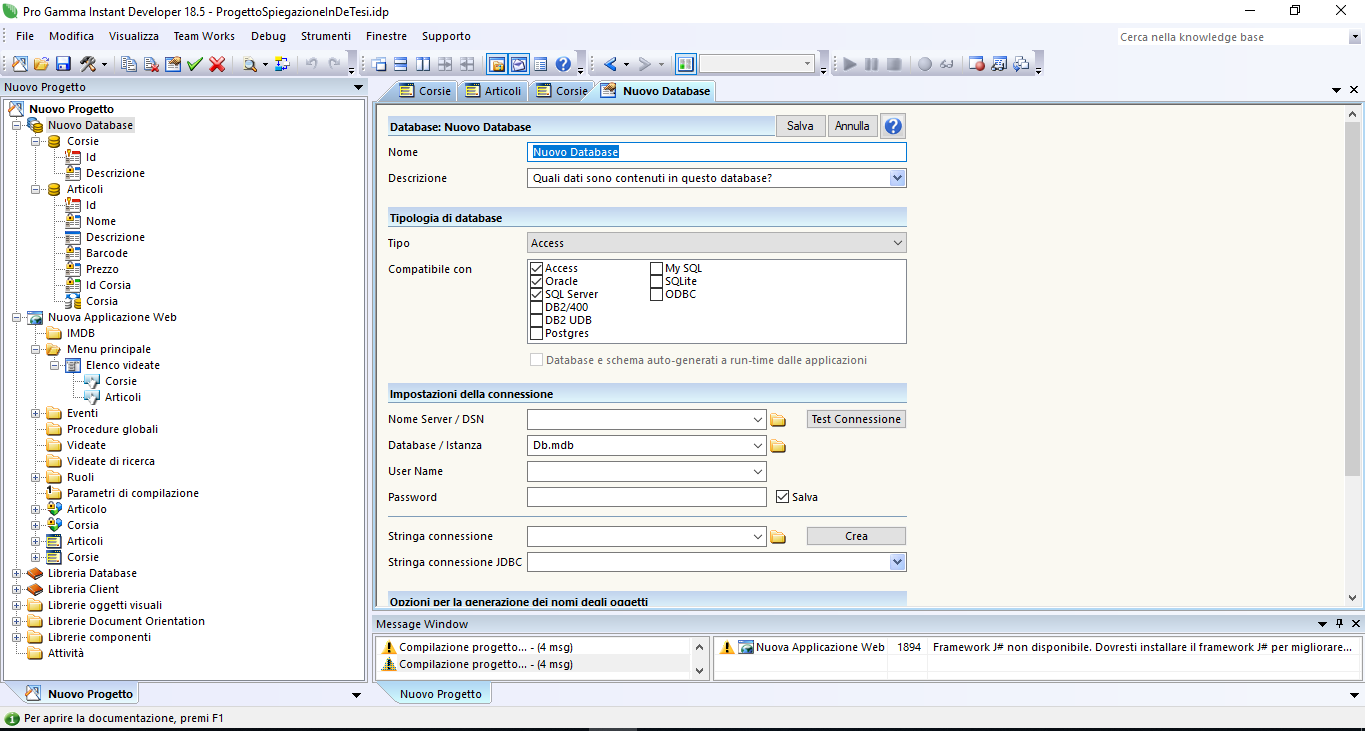
\includegraphics[width=0.49\columnwidth]{InDe_01} 
	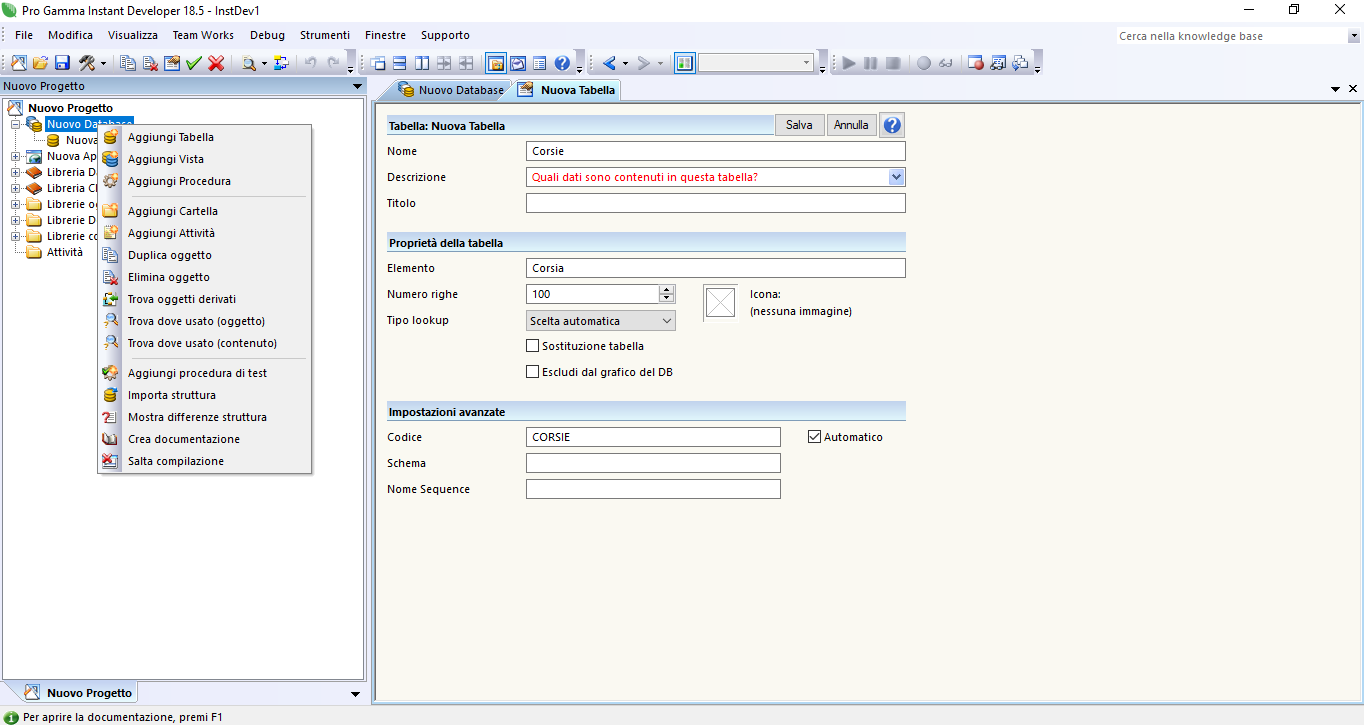
\includegraphics[width=0.49\columnwidth]{InDe_02} 
	\caption{InDe: inserimento proprietà database e tabella}
	\label{InDe_Db_proprietà db_t}
\end{figure}

\begin{figure}[!h] 
	\centering  
	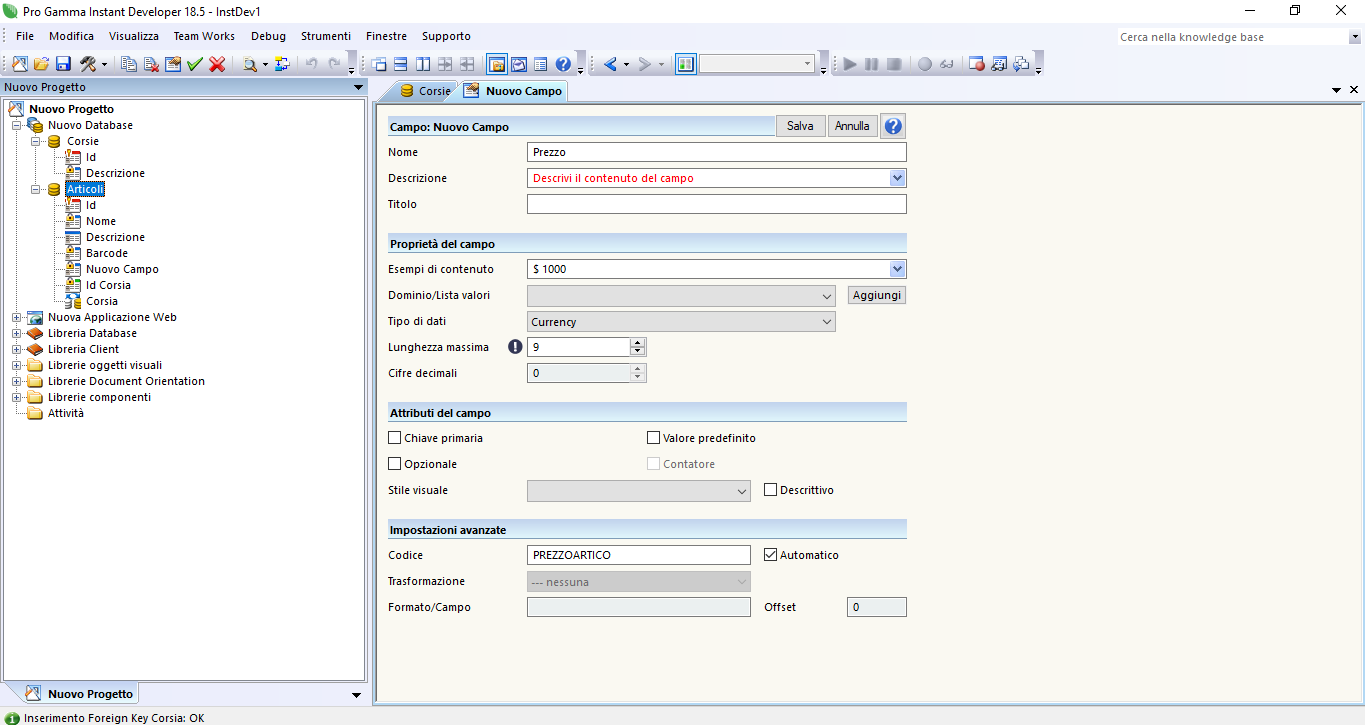
\includegraphics[width=0.49\columnwidth]{InDe_03} 
	\caption{InDe: inserimento proprietà degli attributi della tabella}
	\label{InDe_Db_proprietà_a}
\end{figure}


\subsubsection{Passo 2: Oggetto}
Una volta creata la tabella, per definire un oggetto è sufficiente trascinare sull'applicazione la tabella stessa tenendo premuto shift e ctrl. Viene generato un documento nel quale sarà possibile inserire metodi, modificare eventi e aggiungere campi. Nel caso considerato mi limito a creare l'oggetto.

\begin{figure}[!h] 
	\centering  
	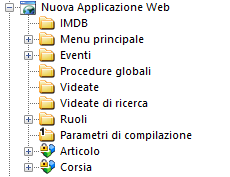
\includegraphics[width=0.3\columnwidth]{InDe_04} 
	\caption{InDe: creazione di oggetti basati su tabelle}
	\label{InDe_Oggetti}
\end{figure}

\subsubsection{Passo 3: Videata}
Trascinando l'oggetto sull'applicazione e premendo o shift o ctrl viene creata una videata basata sull'oggetto. Selezionando la videata interessata è possibile modificarla graficamente e gestirne le funzionalità. Infine inserendo la videata nella voce dei menù, potrà essere aperta all'esecuzione dell'applicazione.

\begin{figure}[!h] 
	\centering  
	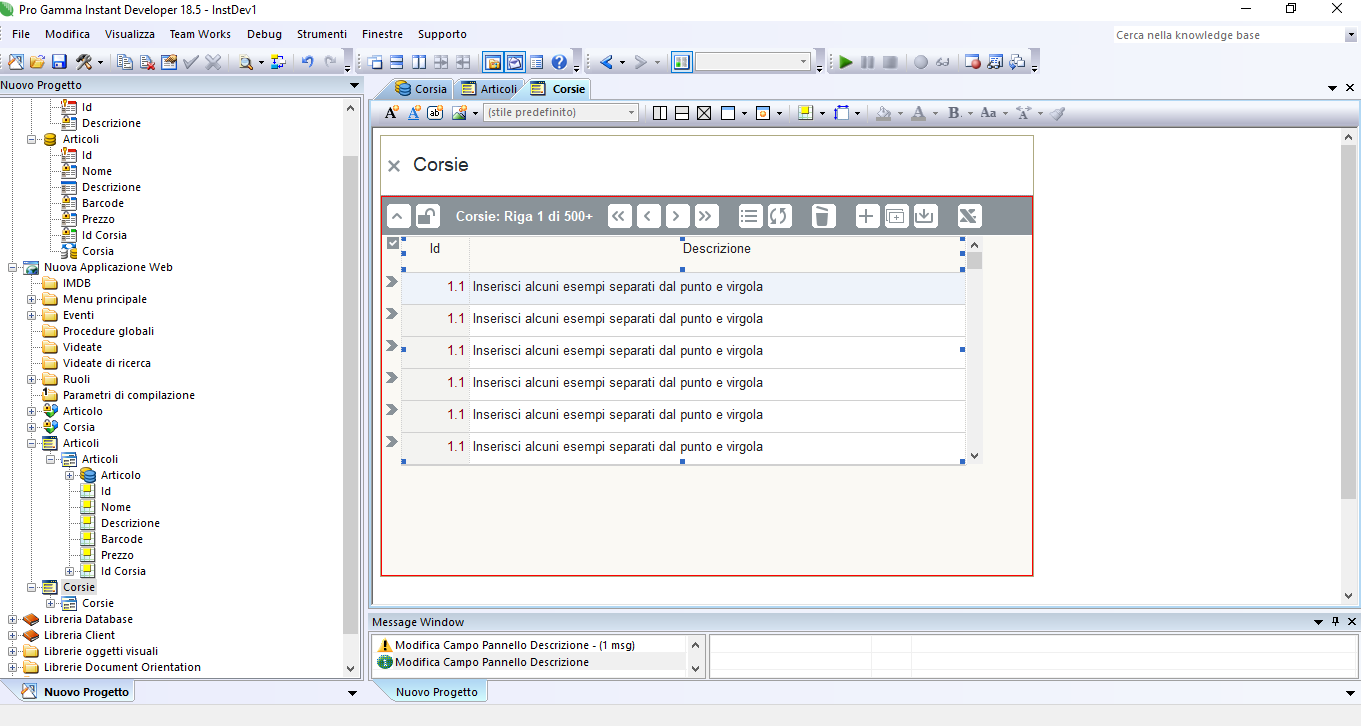
\includegraphics[width=0.49\columnwidth]{InDe_05}
	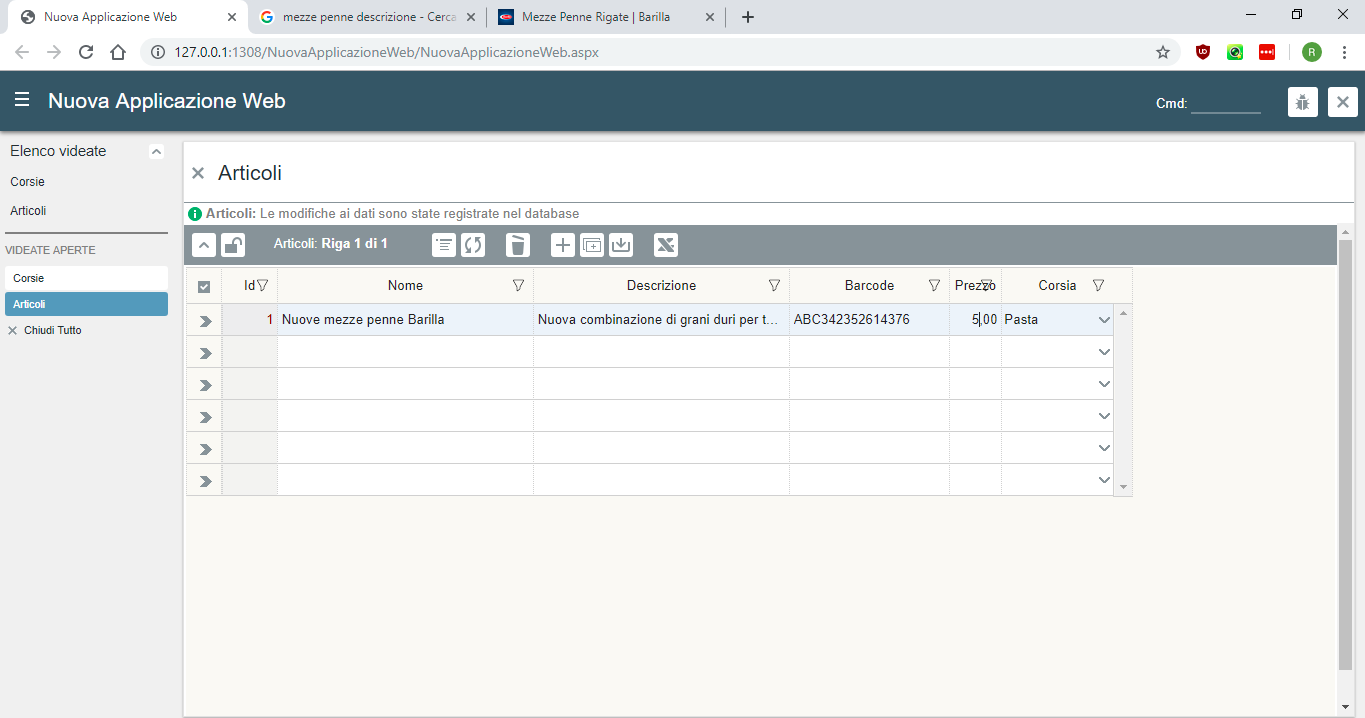
\includegraphics[width=0.49\columnwidth]{InDe_06}
	 
	\caption{InDe: modellazione della videata e risultato finale}
	\label{InDe_videata}
\end{figure}


\subsection{Estensioni}
In questo contesto non è risultato necessario impiegare questa funzionalità. Tuttavia, ritengo importante accennare alle possibilità offerte dall'applicazione. InDe, infatti, permette di estendere le sue librerie con delle nuove. \'E possibile creare delle funzioni in SQL e anche implementare esternamente un file Java o C\# e richiamarlo nell'applicazione adottando le funzioni indicate nella \hyperref[InDe_estensioni]{figura \ref{InDe_estensioni}}. 

L'aspetto negativo delle estensioni è che una volta implementate in Java, C\# o nel linguaggio del database (Oracle, SQL Server, MySQL) non si può cambiare tecnologia, salvo il caso in cui non si siano implementate le estensioni per tutti i linguaggi. 

Le estensioni permettono di realizzare applicazioni personalizzate e con particolarità uniche realizzate per uno specifico linguaggio, tuttavia non sarà possibile passare da un tipo di linguaggio ad un altro fintanto che non si implementa il complementare. Per una azienda con diversi clienti, da software house a produttori di mobili, un prodotto deve essere quanto più standard possibile se questo è a scopo di vendita senza successiva personalizzazione. 

\begin{figure}[!h] 
	\centering  
	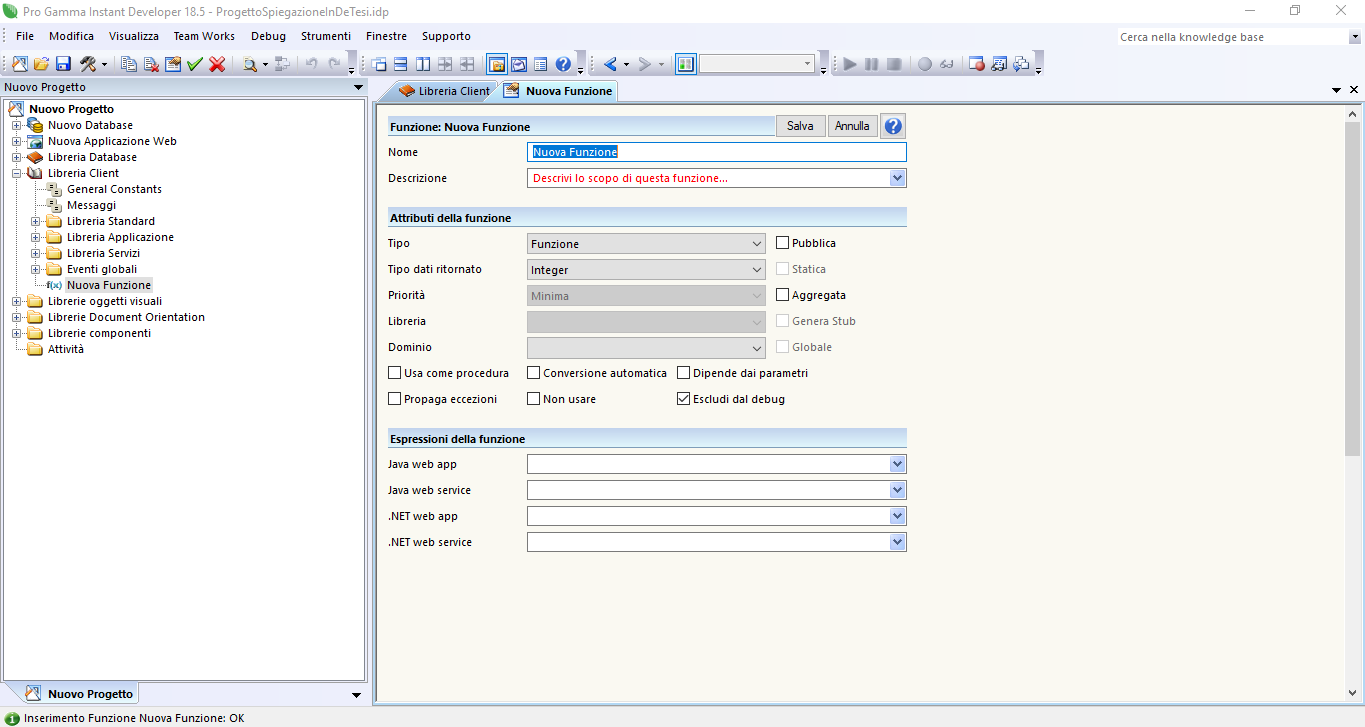
\includegraphics[width=0.49\columnwidth]{InDe_07}
	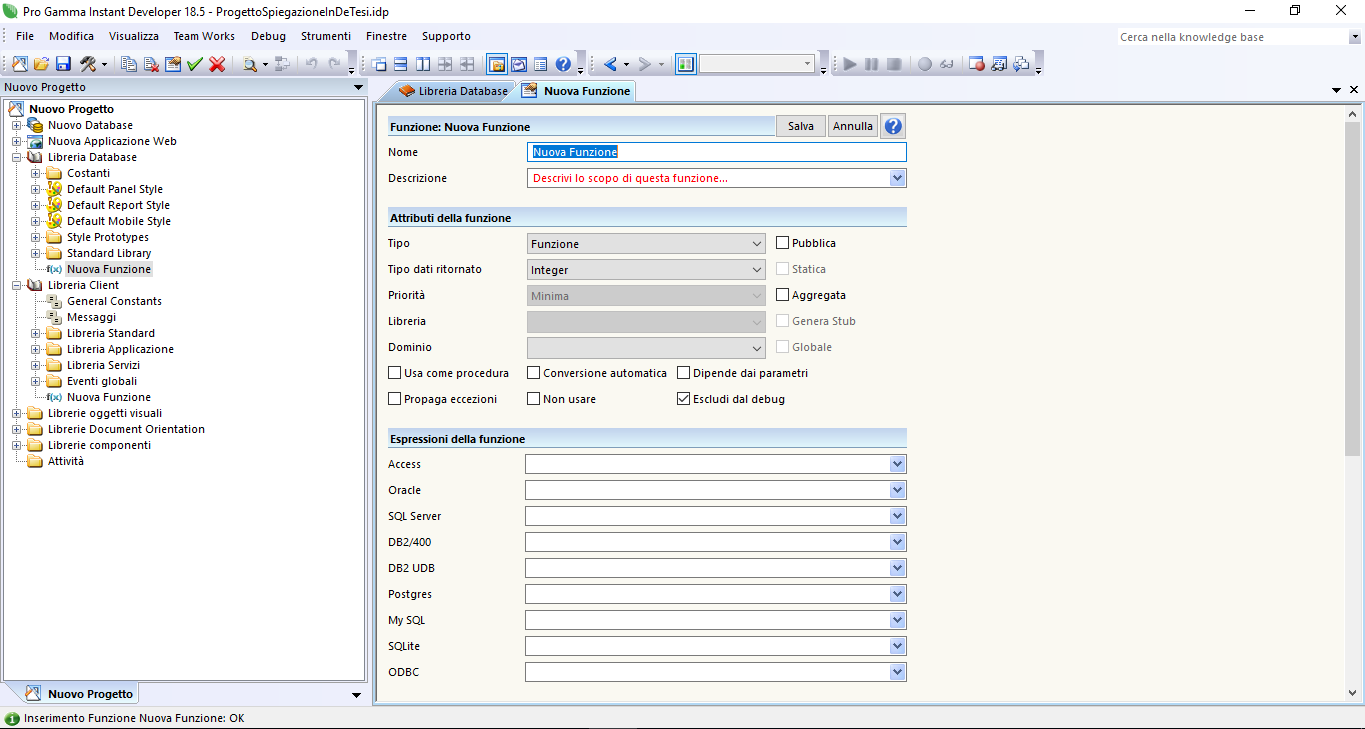
\includegraphics[width=0.49\columnwidth]{InDe_08}
	\caption{InDe: gestione delle estensioni}
	\label{InDe_estensioni}
\end{figure}


\section{Obiettivi}
In questa sezione sono contenuti gli obiettivi di progetto.

\subsection{Stage}
Lo stage si è svolto in 310 ore esattamente come da pianificazione. Le attività hanno avuto tempi diversi rispetto a quanto previsto nel Piano di lavoro: l'apprendimento del software, delle stored procedure e dei formalismi hanno richiesto quattro giorni, permettendomi di anticipare lo studio dell'applicazione, ad oggi, completata.  L'implementazione e il rilascio del progetto hanno richiesto la totalità del tempo lavorativo, non potendo affrontare l'aspetto delle stored procedure. 
La seguente tabella illustra lo stato di soddisfacimento dei requisti:


	\begin{longtable}{ l|l|c }
		\hline
		
		\multicolumn{2}{c}{\textbf{Obbligatori}} & \textbf{Soddisfatto} \\
		\hline
		\textit{O01} & Apprendimento della piattaforma Instant Developer & Si\\
		\textit{O02} & Test delle funzionalità implementate e rilascio & Si\\
		\textit{O03} & Utilizzo di Microsoft SQL Server& Si\\
		\hline
		\newpage
		\hline
		\multicolumn{2}{c}{\textbf{Desiderabili}} & \textbf{Soddisfatto}\\
		\hline
		\textit{D01} & Gestione di progetto & Si\\
		\textit{D02} & Comunicazione con il cliente & Si\\
		\textit{D03} & Scrittura delle procedure T-SQL& No\\
		\hline
		\multicolumn{2}{c}{\textbf{Facoltativi}} & \textbf{Soddisfatto}\\
		\hline
		\textit{F01} & Autonomia a risolvere nuove problematiche & Si\\
\caption{Raggiungimento degli obiettivi di stage}
		
	\end{longtable}
	

\subsection{Personali}
Per quanto riguarda gli obiettivi personali, mi ritengo pienamente soddisfatto. Le attività e le tecniche di programmazione apprese mirano molto sulla logica e meno sul codice. Inoltre, ho potuto osservare alcuni data warehouse e comprendere alcune delle funzionalità e le scelte che portano la realizzazione di alcune delle tabelle. Infine, ho imparato quanto difficile può essere la comunicazione tra cliente e fornitore.
Riassumendo, gli obiettivi personali raggiunti sono:


\begin{table}[h]
	\begin{tabular}{p{10cm}|c}
		\hline
		\textbf{Personali}& \textbf{Soddisfatto} \\
		\hline
		Accrescere le conoscenze in merito al mondo RAD e Data Warehouse & Si\\
		Migliorare le capacità di realizzazione di applicazioni seguendo il metodo Bottom-Up & Migliorabile\\
		Apprendere come interfacciarmi con i clienti & Si\\
		Migliorare le mie capacità di Problem Solving & Si

	\end{tabular}
\caption{Raggiungimento obiettivi personali}
\end{table}


\section{Considerazioni personali}
Ho iniziato a programmare durante le superiori. La mia passione per l'informatica è nata sin dalla creazione delle prime applicazioni. L'aspetto che più mi affascina di questa disciplina è vedere che un programma da me creato sia adoperato da altre persone. Alle superiori, tuttavia, non ho avuto una preparazione completa e ho deciso di intraprendere l'Università cercando di ampliare le mie conoscenze. Appena iniziato il percorso universitario ho subito affrontato delle difficoltà legate alla quantità di studio e all'organizzazione necessaria per affrontare gli esami. Nonostante le difficoltà incontrate, ogni volta che mi fermo a leggere i libri consigliati dai professori rimango attratto dalle capacità e della logica alla base di un programma. 
Alle superiori mi concentravo nel far funzionare una applicazione, con l'università ho appreso che da una buona logica di base è possibile realizzare applicazioni efficienti ed efficaci. Lo stage mi ha portato a ragionare maggiormente sulla logica di una applicazione.

Appena iniziato lo stage, ho affrontato una sessione di studio. Come già ho accennato nella \hyperref[scelta e obiettivi]{sottosezione \ref{scelta e obiettivi}}, lavorare presso \azienda\ mi ha permesso di conciliare du aspetti della mia persona: il ragioniere e l'informatico. Inoltre ho potuto apprendere una metodologia differente da quella a cui ritengo molti studenti siano associati, ovvero un programma è buono solo se si ha il controllo completo su ogni classe e componente. 
Da studente, scrivere codice è entusiasmante, ma si rischia spesso di perdere di vista uno degli obiettivi di un programma, l'efficienza. Da quanto ho osservato sia in Programmazione ad oggetti e Ingegneria del software a seguito di scadenze imminenti spesso si cerca di consegnare un prodotto che esegue quanto specificato a discapito di altri aspetti.

Adesso sono conquistato dalle capacità degli strumenti di sviluppo assistito. In particolare \inde, un programma italiano, che offre la possibilità di concentrare la propria attenzione sulla logica di un programma.  
Con questa mia affermazione non intendo però definire InDe come il migliore. Lavorando con quest'ultimo ho individuato delle funzionalità da migliorare, come nel caso del BeforeSave(). Questo metodo ha tre parametri, uno dei quali è la fase (inserimento, modifica, cancellazione) che può essere usato con uno switch, ciò nonostante si deve creare un blocco if interno ai case di inserimento e modifica nei quali uno esclude l'altro, altrimenti l'applicazione esegue entrambe le operazioni.\\

L'\myUni\ mi ha permesso di arrivare preparato alla mia prima esperienza lavorativa. Ritengo che la conclusione degli studi con lo stage obbligatorio sia il modo più efficacie di preparare uno studente al futuro, sia che scelga di continuare gli studi, sia che decida di iniziare a lavorare. Relazioni con aziende, come nel caso dello stage e del corso di Ingegneria del software, sono fondamentali e permettono di ampliare il proprio pensiero molto spesso radicato in un'ambito accademico. 

A mio parere, il corso di studi offerto è ottimale ed in combinazione con i progetti realizzati nella triennale, ho acquisito le capacità che mi hanno permesso di integrarmi al team di sviluppo dell'azienda ed a interagire con i clienti. 
 